基于以上设备所需要实现的五大基本功能,我们可以得出凡是基于VxWorks内核调用的驱动程序不外乎以下的组成部分:

\begin{enumerate}
\item 设备驱动函数的注册函数。驱动开发人员必须要开发响应的函数将驱动程序的功能注册到设备驱动程序列表中,以便挂接到I/O系统。

\item 设备驱动的卸载函数。若系统不再使用设备,需要将其卸载掉,以节约系统资源

\item 设备的打开和关闭函数。这两个函数是相伴的,有打开操作就必须有关闭操作。

\item 设备的读写函数。主要完成设备的外设和CPU之间的数据交换。

\item 设备的控制函数。在使用设备的过程中,需要对设备的工作状态进行控制。

\item 中断服务函数(ISR)。响应外设的中断请求。
\end{enumerate}\\



\textsc{%此处集成开发环境应该将其删除,或者将移到其他的部分来简单的介绍。
\section{集成开发环境Tornado}

	Tornado是嵌入式实时领域里最新一代的开发调试环境,其系统结构如\autoref{fig:Tornado开发系统结构}所示。Tornado提供了高效明晰的图形化的实时应用开发平台,可以帮助轻松的完成程序的编辑、编译、调试、系统配置等工作。它包括一整套完整的面向嵌入式系统的开发和调试工具。Tornado采用的是主机—目标机的交叉开发模型,应用程序在主机的Windows环境下编译链接生成可执行文件,下载到目标机,通过主机上的目标服务器与目标机上的代理程序的通信完成对应用程序的调测、分析。这些工具包括C和C++远程级调试器、目标和工具管理、系统目标跟踪、内存使用分析和自动配置,所有工具都能够很方便的同时运行,很容易增加扩展和交互式开发。
\begin{figure}[!h]	
\centering
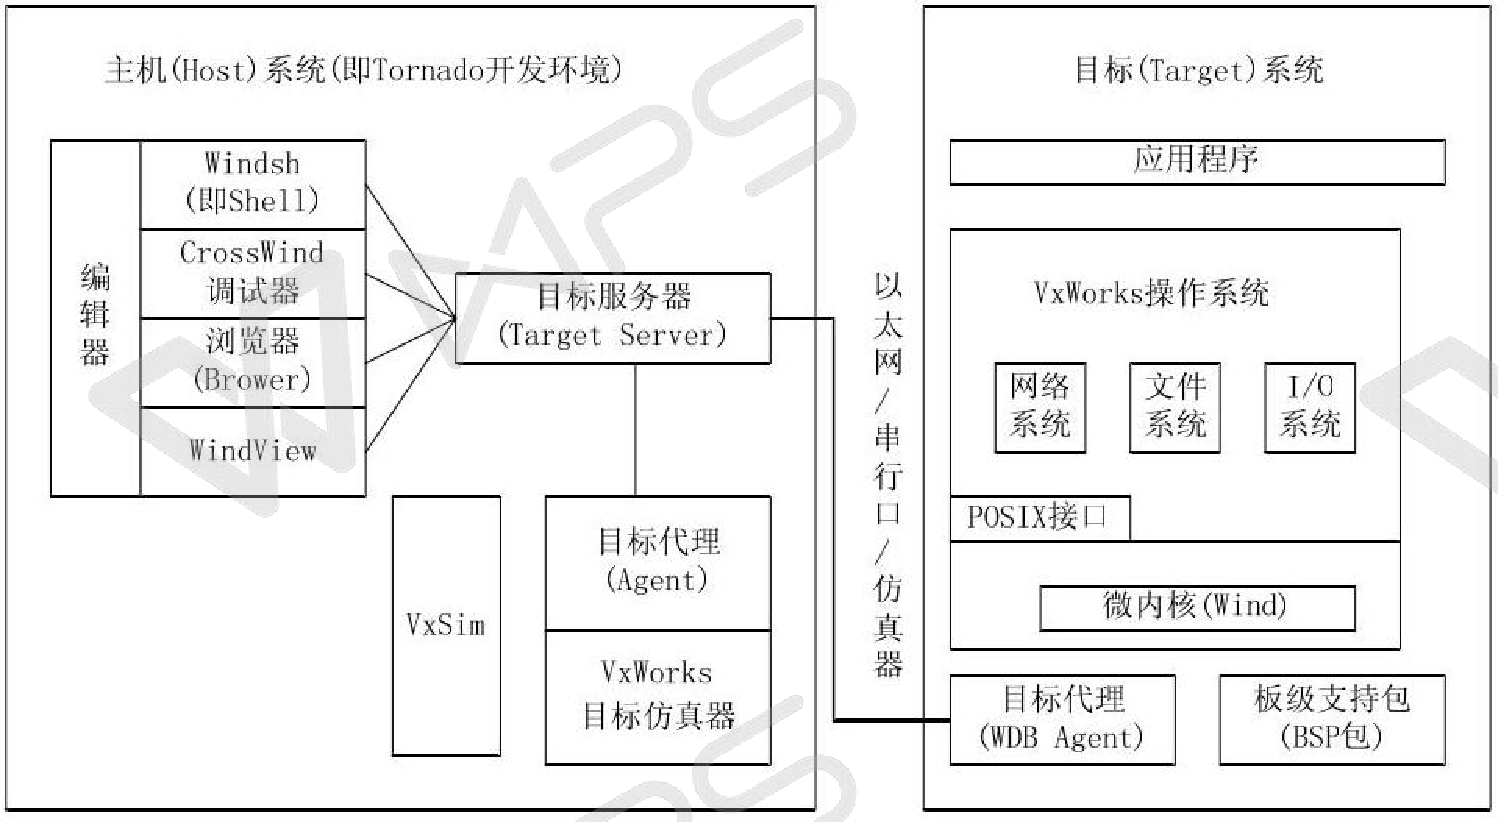
\includegraphics[width=1.0\textwidth]{./graphics/tornado-system-structure.pdf}
\caption{Tornado开发系统结构}\label{fig:Tornado开发系统结构}
\end{figure}
	
	典型的主机开发系统通常有比较大的RAM、硬盘空间、打印机以及其他外部设备,而典型的目标机系统只有仅能满足实时应用的资源,除此以外可能还有比较少量的用于测试和调试的额外资源。Tornado开发环境的基本优点是应用模块不需要链接到运行系统库。Tornado直接装载重定位的目标模块,通过每个模块里的符号表来动态解析外部符号的引用,解析符号表是由运行在目标机上的目标服务器来完成的。Tornado在开发过程中会把目标模块的大小减到最小,这样可以缩短开发周期。主机端驻留的shell和调试器也能够调用和测试独立的应用程序或者是完整的任务。

	Tornado是为开发VxWorks应用程序提供的集成开发环境,其中包含有工程管理软件,可以将用户自己的代码和VxWorks的核心有效的结合起来,可以按照用户的需要裁剪配置VxWorks内核;
Tornado开发系统包含有三个高度集成的部分:
\begin{itemize}
\item \hei{运行在宿主机和目标机上的强有力的交叉开发工具和实用程序;}
\item \hei{运行在目标机上的高性能、可裁剪的实时操作系统VxWorks;}
\item \hei{连接宿主机和目标机的多种通信方式,如以太网,串口线,ICE或ROM仿真器等。} 
\end{itemize}

Tornado主机集成开发环境中的主要工具为:
\begin{itemize}
\item \textbf{工程管理和配置工具:} 提供工作空间用于应用程序的组织和管理,可通过图形化的配置工具对VxWorks及其组件进行配置。
\item \textbf{交叉编译器:} 提供GNU和Diab两种交叉编译器和类库
\item \textbf{调试器:}提供图形界面的调试方式,可以通过编辑窗口的右键菜单来设置断点和查看变量;
\item \textbf{WindSh:} 一个驻留在主机端的命令行解释器,提供从主机端控制所有运行系统的接口
\item \textbf{CrossWind调试器:}一个远程源码级的调试器,该调试器控制窗口综合了GDB命令行接口和WindSh工具。
\item \textbf{浏览器:} 是一个系统对象的查看器,可以监视目标机的状态。
\item \textbf{WindView逻辑分析器:} 一个动态可视化工具,可以提供上下文切换的情况,事件和有关测量对象的信息。
\item \textbf{VxSim仿真器:} 用来模拟目标操作系统。
\end{itemize}

	位于主机上的目标服务器和位于目标机上的目标代理通过WDB(Wind Debug)协议完成主机和目标机之间的通信。二者无论采取哪种链接方式,都是基于WDB协议的。

	
		
	方便编程人员对系统进行分析、调试。同时基于应用程序的可移植性的考虑,VxWorks在其内核Wind中也支持 POSIX 1003.1b的规定和1003.1中有关基本系统调用的规定,包括:过程初始化、文件与目录、I/O 初始化、语言服务、目录处理;而且 VxWorks 还支持 POSIX 1003.1b的实时扩展,主要包括:异步 I/O、记数信号量、消息队列、信号、内存管理和调度控制等\cite{Wind2003VxWorks}。当然有些POSIX接口也有VxWorks下的实现重新实现版本,比如定时器、二进制信号量、消息队列等。VxWorks下专用的实现版本和POSIX兼容的实现版本在性能上有一些差异,POSIX的接口主要是为简化Linux下程序的移植而设立的。对于没有POSIX接口的部分则必须将程序修改为VxWorks下的接口,对于修改了的代码在VxWorks下运行可能会出现各种问题,本文为了给出一个事后对程序进行分析的方法,于是设计了这个基于VxWorks下的调试通道。



	串口因为其简单可靠、使用方便、开发成本较低等优点\cite{串口调试}。 数据传输是现代通讯过程中的一个重要环节,在数据的传输过程中,不仅仅要求数据传输的准确率要高,而且要求速度快,连接方便。传统的RS232串口通讯和并口通讯都存在传输速度低,扩展性性差、安装麻烦等缺点,而基于USB接口的数据传输系统能够较好的解决这些问题。目前USB接口以其传输速率高、即插即用、支持热插拔等优点,逐步成为PC机的标准接口。PC端的应用软件依然是针对串口进行编程,外设也是以串口为数据通道,但是从PC到外设的物理连接使用的却是USB总线,在上的数据通信也是USB数据格式。

	对于特性相异的设备要使用串行通信来连接时,必须保证双方所使用的的标准接口是一致的。一般的串口标准有RS-232、RS-485、TTL等。从通信的方向性来看,串口通信有单工、半双工和全双工三种方式。单工通常使用一根导线,通信只在一个方向进行,如监视器、打印机、电视机。半双工可以在两个方向上进行,但是方向切换时有时间延迟,如打印机。全双工可以在两个方向上运行,且时间的切换没有时间延迟,适用于那些不能有时间延迟的交互式应用,如远程监控等。






\begin{enumerate}
\item \hei{USB设备与主机系统的交互}

	MCU对USB芯片进行初始化:设置内部时钟,选择内部连接方式以及是否开通DMA传输等;设定设备的工作模式,并设备本设备的初始地址为0(USB规范指明当设备接入PC的时候都由初始为0的地址对主机进行响应,之后再由主机分配一个地址给USB设备,设备接收到分配地址命令后,再更改自己的地址,并一直通过这个地址完成后续的通信)。
	完成初始化工作之后,MCU将使能USB接口,主机系统将因此检测到一个新的USB接入而很快与设备进行握手,获取设备的基本信息,并完成一些列的对设备的配置,其过程为:
	\begin{enumerate}
	\item USB上电使能后,主机会向USB设备发送GET DEVICE DESCRIPTOR的命令,之后主机会收到设备发出的设备描述符,随即为设备分配一个空闲地址,并向设备发送SET ADDRESS的命令,这时设备通过地址0发送一个长度为0的数据包予以应答,然后根据主机的要求更改自身的地址,而且这以后的数据交换都将会通过这个新的地址来进行。
	\item 完成地址设备之后,主机将会发送GET CONFIGURATION DESCRIPTOR,USB规定当主机发出该命令符的时候,设备必须要同时返回配置所包含的所有接口和接口所包含的所有端点的描述符。
	\item 主机获取到USB设备的描述符、配置描述符并进行了地址设置之后,设备与主机的握手初步完成,之后会将该设备加入到设备列表当中。
	\end{enumerate}
	
	\item \hei{USB设备与驱动程序的交互}
	
USB设备的驱动与传统意义上的硬件驱动不完全相同,他并不与硬件直接通信,而是以创建和发送URB请求块的形式把命令传递给操作系统所提供的USB总线驱动程序,由总线驱动程序来完成与硬件的直接交互。和主机类似,驱动会首先创建和发送请求得到该设备的DEVICE DESCRIPTOR的URB,并将获取到的信息存储在专用的数据结构当中,接着驱动为了得到完整的设备配置,必须要通过总线驱动发送两次GET CONGFIGURATION DESCRIPTOR命令得到设备。获取设备的配置信息之后,驱动在启动设备之前还要发送SET CONFIGURATION、SET INTERFACE命令。通过以上的几个步骤便可以完成驱动与USB设备过程。	
\end{enumerate}



实时操作系统(Real Time Operation System,简称RTOS)是整个实时系统的核心。POSIX1003.1标准为RTOS下了一个简单的定义:RTOS是能够在有限的响应时间内为应用提供所要求级别服务的操作系统\cite{Renard20081003}。当外界事件或者是数据产生时,RTOS需要快速的进行处理,并且处理的结果又能够在规定的时间之内来控制生产过程或者对处理系统做出快速的响应,调度一切可利用的资源来完成实时任务。实时系统按照实时的效果可以分为软实时和硬实时,硬实时要求在规定的时间内必须完成操作,这是通过操作的在设计的时候就得到保证的;软实时只需要按照任务的优先级,尽可能快的完成任务即可。\\
一个实时操作系统的特征通常包括以下几点:
\begin{itemize}
\item \textbf{高精度计时系统}\\
	计时精度是影响实时性的一个重要因素,在实时系统当中,经常需要精确确定实时地操作某个设备或执行某个任务,或精确的计算一个时间函数。这些不仅仅依赖于一些硬件提供的时钟精度,也依赖于实时操作系统的高精度计时功能。
\item \textbf{多级中断机制}\\
	中断是实时操作系统当中的一个关键设施,是用于通知系统发生外部事件的常用机制。一个实时操作系统通常需要处理多种外部信息或事件,但处理的紧迫程度有轻重缓急之分。有的必须立即作出反应,有的则可以延后处理。因此,需要建立多级中断嵌套处理机制,以确保对紧迫程度较高的实时事件进行及时响应和处理。
\item \textbf{实时调度机制}\\
	实时操作系统不仅要及时响应实时事件中断,同时也要及时调度运行实时任务。但是,处理机调度并不能随心所欲的进行,因为涉及到两个进程之间的切换,只能在确保“安全切换”的时间点上进行,实时调度机制包括两个方面,一是在调度策略和算法上保证优先调度实时任务;二是建立更多“安全切换”时间点,保证及时调度实时任务。
\end{itemize}
本次所需完成的调试通道正是基于一个目前业界有名的实时操作系统VxWorks。






\subsection{VxWorks下驱动程序的开发}
	
	VxWorks作为一款嵌入式操作系统,为了屏蔽硬件的具体操作细节,为上层应用程序提供统一的接口,引入了设备驱动程序的概念。设备驱动程序是用来直接控制设备,以完成设备应有的操作。操作系统通过驱动程序来对设备进行操作,属于一种软件接口。这样,应用程序开发使用统一的软件接口,使得开发人员可以专注于应用程序的开发,不用考虑底层的物理设备。
	
	VxWorks操作系统下的驱动程序在其开发上有自身规范,且对于不同的设备的驱动程序开发也表现出较大的差异。嵌入式设备的硬件平台千差万别,厂商不可能遇见所有的设备并提供相应的驱动程序,因此要实现VxWorks的跨平台移植,用户必须要根据硬件平台开发驱动程序。所以,开发VxWorks操作系统下外围设备的驱动程序具有很大的实际应用价值。
		
	虽然VxWorks作为实时嵌入式系统有着无比强大的性能表现,但是就目前的现状来看,VxWorks操作系统的平台成本很高,因为VxWorks是一个专用系统,使用这个系统的单位或公司都是处于军事,航天等特殊行业当中,这使得他们的开发经验和资源不能够拿出来共享,导致VxWorks的参考资料比较少,没有成熟活跃的社区支持,且VxWorks并不是一个开源的系统,需要花不菲的价格进行购买和售后支持,这些都提高了VxWorks的应用的开发门槛,使得一般的开发人员不能够方便的接入到对其的应用研究当中,增加了开发难度。
	
	





	VxWorks系统主要如下几个组件,一般的应用程序也就用到如下几个模块:任务调度负责任务优先级,任务创建,任务删除等功能。任务通讯主要涉及队列管理,管道管理等。IO管理就是通用外设的输入输出管理。文件管理包含文件或者链接创建,修改,删除,检索等等。内存管理包含内存申请及内存释放。定时器管理就是定时器创建,定时器删除。网络通信包含套接字创建,udp/tcp通信,套接字删除,及配置管理。同步就是任务同步。互斥就是任务互斥,保护关键资源。
	
	在VxWorks操作系统的代码架构里面,一般写一个应用程序只需要涉及上面几个系统组件,由于VxWorks操作系统组件化非常好,这几个组件的耦合度非常低,每个组件对外提供都是单独的头文件,比如任务调度,其头文件为taskLib.h,任务通讯如果用的队列,那其头文件就是msgQLib.h,如果是定时器管理,那其头文件就是timerLib.h,因此也让程序移植提供了很大的便利性。有很多人认为,VxWorks跟Linux操作性的系统头文件差异化太大,因此移植难度成倍速增加,其实不然,就是由于VxWorks的高度组件化,让程序移植提供了很大的便利性。
	
	
	wind使用中断驱动和优先级的方式。它缩短了上下文转换的时间开销和中断的时间延迟。VxWorks中的任何例程都可以被启动为一个单独的任务,拥有它自己的上下文和堆栈,还有一些其他的任务机制可以使得任务挂起、继续、删除、延时或改变优先级。	
	
	
	板级支持包BSP(Board Support Package)作为VxWorks系统的主要组成部分,对各种板子的硬件功能提供了同一的软件接口,它包括硬件初始化、中断的产生和处理、硬件时钟和计时器管理、局域和总线内存地址映射、内存分配等。每一个板级支持包包括一个ROM启动(Boot ROM)或其他启动机制。

% appendix环境用于附录环境。即可以将附录置于appendix环境当中。如:
% \begin{appendix}
%  <content>
% \end{appendix}

% 直接使用\appendix 则表明后文均为附录。如:
% \appendix
%  <content> 
\appendix

% publications环境用于已经发表了的论文的页面,一般用于附录当中,使用上同enumerate环境
\begin{publications}
    \item 论文1
    \item 论文2
\end{publications}

\chapter{这是一个附录}\label{appendix:1}
附录正文。


%\subsection{第二层}\label{sec:1}
%\subsubsection{第三层}\label{sec:1}
%测试测试测试测试测试测试测试测试测试测试测试测试。
%\footnote{\label{footnote:1}脚注}

\section{字体}

普通\textbf{粗体}\emph{斜体}

\hei{黑体}\kai{楷体}\fangsong{仿宋}

\section{公式}

单个公式,公式引用:\autoref{eq:1}。
\begin{equation}
 c^2 = a^2 + b^2 \label{eq:1}
\end{equation}

多个公式,公式引用:\autoref{eq:2},\autoref{eq:3}。

\begin{subequations}
\begin{equation}
  F = ma \label{eq:2}
\end{equation}
\begin{equation}
  E = mc^2 \label{eq:3}
\end{equation}
\end{subequations}

\section{罗列环境}

\begin{enumerate}
    \item 第一层\label{item:1}
    \item 第一层
    \begin{enumerate}
        \item 第二层\label{item:2}
        \item 第二层
        \begin{enumerate}
            \item 第三层\label{item:3}
            \item 第三层
        \end{enumerate}
    \end{enumerate}
\end{enumerate}

\begin{description}
    \item[解释环境]  解释内容
\end{description}



\clearpage

\section{代码环境}

\begin{lstlisting}[language=python]
import os

def main():
    '''
    doc here
    '''
    print 'hello, world' # Abc
    print 'hello, 中文' # 中文
\end{lstlisting}

\section{定律证明环境}

\begin{definition}
这是一个定义。
\end{definition}
\begin{proposition}
这是一个命题。
\end{proposition}
\begin{axiom}
这是一个公理。
\end{axiom}
\begin{lemma}
这是一个引理。
\end{lemma}

\begin{theorem}
这是一个定理。
\end{theorem}
\begin{proof}
这是一个证明。
\end{proof}

\section{算法环境}

\begin{algorithm}[H]
\SetAlgoLined
\KwData{this text}
\KwResult{how to write algorithm with \LaTeX2e }
initialization\;\label{alg_line:1}
\While{not at end of this document}{
read current\;
\eIf{understand}{
go to next section\;
current section becomes this
 one\;
}{
go back to the beginning of current section\;
}
}
\caption{How to write algorithms}\label{alg:1}
\end{algorithm}


\section{表格}
表格见\autoref{tab:1}。

\begin{table}[!h]
\centering
\caption{一个表格}\label{tab:1}
\begin{tabular}{|c|c|}
\hline
a & b \\
\hline
c & d \\
\hline
\end{tabular}
\end{table}
\section{图片}
图片见\autoref{fig:1}。图片格式支持eps,png,pdf等。多个图片见\autoref{fig:2},分开引用:\autoref{fig:2-1},\autoref{fig:2-2}。

\begin{figure}[!h]
\centering

\includegraphics[width=.4\textwidth]{hust-title.pdf}
\caption{hust-title}\label{fig:hust-title}
\end{figure}

\begin{figure}[!h]
\centering
  \begin{subfigure}[b]{0.3\textwidth}
  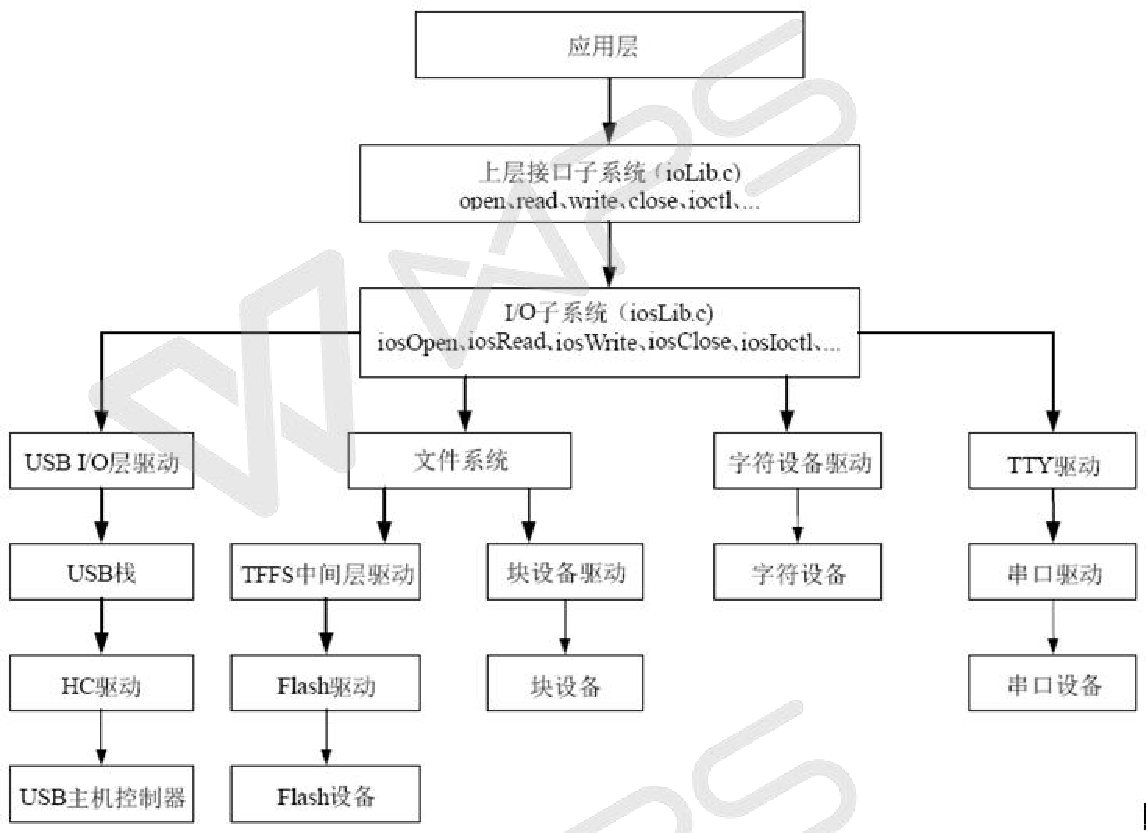
\includegraphics[width=\textwidth]{./graphics/VxWorks-driver-structure.pdf}
  \caption{VxWorks-driver-structure}
  \end{subfigure}
  ~
  \begin{subfigure}[b]{0.3\textwidth}
  \includegraphics[width=\textwidth]{}
  \caption{图片2}\label{fig:2-2}
  \end{subfigure}
\caption{多个图片}\label{fig:2}
\end{figure}

\section{参考文献示例}
这是一篇中文参考文献\cite{徐媛媛2003嵌入式实时操作系统的设备驱动};这是一篇英文参考文献\cite{9787508342894};同时引用\cite{9780124467422,bamboosilk}。

\section[\textbackslash{}autoref 测试]{\texttt{\textbackslash{}autoref} 测试}

\begin{description}
  \item[公式] \autoref{eq:1}
  \item[脚注] \autoref{footnote:1}
  \item[项] \autoref{item:1},\autoref{item:2},\autoref{item:3}
  \item[图] \autoref{fig:1}
  \item[表] \autoref{tab:1}
  \item[附录] \autoref{appendix:1}
  \item[章] \autoref{chapter:1}
  \item[小节] \autoref{sec:1},\autoref{sec:2},\autoref{sec:3}
  \item[算法] \autoref{alg:1},\autoref{alg_line:1}
  \item[证明环境] \autoref{def:1},\autoref{proposition:1},\autoref{axiom:1},\autoref{lemma:1},\autoref{theorem:1},\autoref{proof:1}
\end{description}}